\documentclass[11pt]{article}

% ---- arXiv-safe packages ----
\usepackage[utf8]{inputenc}
\usepackage[T1]{fontenc}
\usepackage{newtxtext,newtxmath}
\usepackage{amsmath}
% amssymb omitted: newtxmath provides equivalent coverage
\usepackage{graphicx}
\usepackage{booktabs}
\usepackage{makecell}
\usepackage{hyperref}
\usepackage{caption}
\usepackage{subcaption}
\usepackage[noend]{algpseudocode}
\usepackage{algorithm}
\usepackage{tikz}
\usepackage{pgfplots}
\usepackage{pgfplotstable}
\pgfplotsset{compat=1.18}
\usetikzlibrary{positioning, shapes.geometric, arrows.meta, fit, calc}

% ---- hyperref setup ----
\hypersetup{
  colorlinks=true,
  linkcolor=blue,
  citecolor=blue,
  urlcolor=blue,
  breaklinks=true
}

% ---- title ----
\title{NanoForecast v0.5:\\Competitive Time Series Forecasting Through\\Training Pipeline Optimization}

\author{Gautam Kishore \\
Eulogik, Inc. \\
\texttt{gautam@eulogik.com} \\
\url{https://eulogik.com}
}

% ---- begin ----
\begin{document}

\maketitle

% ==========================================================================
\begin{abstract}
We present NanoForecast v0.5, a lightweight time series forecasting model (6.5M parameters) that achieves competitive accuracy with models up to 109$\times$ larger through systematic training pipeline refinement. Retraining the unchanged v0.3 architecture with a corrected pipeline (loss-scope handling, tensor shape alignment, and expanded augmentation coverage) improves overall Mean Absolute Scaled Error by 46.6\% under a standard protocol (MASE 3.282 $\to$ 1.752), with zero architecture modifications and the same data and compute budget. Despite being 31$\times$ smaller than TimesFM (200M parameters), NanoForecast v0.5 outperforms it on all three ETT datasets (MASE 0.685/1.109/0.289 vs.\ 0.705/1.360/0.545) and comes within 1\% on exchange rate; TimesFM dominates on the high-cardinality electricity and traffic sets. Against PatchTST (15M+ parameters, official thuml configuration), NanoForecast wins on all three ETT sets. The model trains on a single cloud GPU (NVIDIA T4, Google Colab) in approximately 12 hours and runs on edge hardware (Raspberry Pi 4, \$35 USD) without GPU requirements. We release all code, pretrained checkpoints, and evaluation framework under Apache 2.0 at \url{https://github.com/eulogik/NanoForecast}.
\end{abstract}

% ==========================================================================
\section{Introduction}
\label{sec:intro}

Time series forecasting is fundamental to numerous domains including energy management~\cite{ett}, financial modeling~\cite{finance_review}, and supply chain optimization~\cite{supply_chain}. Recent advances in foundation models---TimesFM~\cite{timesfm} (200M parameters), Chronos~\cite{chronos} (710M parameters), and PatchTST~\cite{patchtst} (15M+ parameters)---have demonstrated strong performance on standard benchmarks. However, these models require significant computational resources for both training and inference, limiting their accessibility for practitioners without dedicated GPU infrastructure.

We address a complementary problem: \emph{deployable time series forecasting}. The objective is to achieve competitive accuracy while remaining trainable on consumer hardware and deployable on resource-constrained devices. This requires balancing accuracy, model size, and deployment flexibility---a tradeoff that large foundation models do not currently address.

Our primary contribution is empirical rather than architectural. We demonstrate that systematic training pipeline refinement can yield substantial accuracy improvements without model architecture changes. Starting from the released NanoForecast v0.3 checkpoint (MASE 3.282 under the standard protocol of Section~\ref{sec:setup}, 6.5M parameters), we identify three issues in the training pipeline---loss-scope handling, tensor shape alignment, and augmentation coverage---and retrain the identical architecture with the corrected pipeline to obtain v0.5 (MASE 1.752), a 46.6\% improvement.

Additionally, we show that a 6.5M parameter model can outperform models up to 109$\times$ larger on specific benchmarks: it outperforms TimesFM (200M parameters) on the three ETT datasets (ETTh1, ETTh2, ETTm1) and comes within 1\% of it on exchange rate, and it outperforms PatchTST (15M+ parameters) on all three ETT sets.

\subsection{Contributions}
\label{sec:contributions}

\begin{enumerate}
\item We identify and document three training pipeline issues---loss-scope handling, tensor shape alignment, and augmentation coverage---that silently degrade time series forecasting accuracy, and quantify their joint effect on released checkpoints under a standard protocol.
\item We achieve a 46.6\% MASE improvement (3.282 $\to$ 1.752) through training pipeline refinement alone, with no architecture modifications.
\item We demonstrate that a 6.5M parameter model can outperform models up to 109$\times$ larger on specific benchmarks: outperforming TimesFM (200M parameters) on the three ETT datasets (ETTh1 MASE 0.685 vs.\ 0.705, ETTh2 1.109 vs.\ 1.360, ETTm1 0.289 vs.\ 0.545) and coming within 1\% of TimesFM on exchange rate (4.418 vs.\ 4.383), while outperforming PatchTST (15M+ parameters) on all three ETT sets.
\item We provide a complete production deployment pipeline including ONNX export (27.9\,MB FP32, 9.2\,MB INT8), Docker containers, and stateful streaming inference, enabling training on a single cloud GPU (T4, Google Colab) and inference on edge hardware (\$35 USD).
\end{enumerate}

% ==========================================================================
\section{Problem Formulation}
\label{sec:problem}

We address univariate time series forecasting. Given a context window $\mathbf{x}_{t-C+1:t} = [x_{t-C+1}, \ldots, x_t] \in \mathbb{R}^C$ of $C$ consecutive observations, the task is to predict $H$ future values $\mathbf{y}_{t+1:t+H} = [y_{t+1}, \ldots, y_{t+H}] \in \mathbb{R}^H$, where $H$ is the forecast horizon.

The model produces both point forecasts $\hat{\mathbf{y}} \in \mathbb{R}^H$ and quantile estimates $\{\hat{\mathbf{y}}^{(p)}\}_{p \in \mathcal{P}}$ for a set of probability levels $\mathcal{P} = \{0.1, 0.25, 0.5, 0.75, 0.9\}$, satisfying the monotonicity constraint $\hat{y}^{(0.1)}_t \leq \hat{y}^{(0.25)}_t \leq \ldots \leq \hat{y}^{(0.9)}_t$ for each $t$.

We evaluate using Mean Absolute Scaled Error (MASE)~\cite{mase}:
\begin{equation}
\text{MASE} = \frac{\frac{1}{H} \sum_{t=1}^{H} |y_t - \hat{y}_t|}{\frac{1}{T-s} \sum_{i=s+1}^{T} |x_i - x_{i-s}|}
\label{eq:mase}
\end{equation}
where the denominator is the in-sample mean absolute error of the seasonal-naive (lag-$s$) forecast computed over the training segment of each series, with $s=24$ for hourly data (ETTh, Electricity, Traffic), $s=96$ for 15-minute data (ETTm), and $s=7$ for daily data (Exchange). This scaling follows the convention of the Chronos benchmark~\cite{chronos}. MASE is scale-invariant and enables fair comparison across datasets.\footnote{We report MSE and MAE in the supplementary materials; MASE is the primary metric. All models---including all baselines---are evaluated under the identical protocol defined in Section~\ref{sec:setup}: same splits, same windows, same scaling denominator.} We further note that the released checkpoints are trained for horizon $H=48$; all comparisons in this paper use $H=48$.

% ==========================================================================
\section{Related Work}
\label{sec:related}

\paragraph{Foundation models for time series.}
TimesFM~\cite{timesfm} employs a decoder-only transformer with 200M parameters trained on approximately 100B time points. Chronos~\cite{chronos} tokenizes time series values and fine-tunes T5 (710M parameters). Timer~\cite{timer} uses a generative pre-trained transformer for time series. Lag-Llama~\cite{lagllama} adapts LLaMA for probabilistic forecasting. More recent foundation models include Moirai~\cite{moirai}, Chronos-Bolt~\cite{chronosbolt}, and TimesFM 2.x~\cite{timesfm2}, and the GIFT-Eval benchmark~\cite{gifteval} provides standardized cross-model zero-shot evaluation. These models achieve strong zero-shot performance but require GPU infrastructure for both training and inference and do not support streaming deployment.

\paragraph{Efficient architectures.}
N-BEATS~\cite{nbeats} uses interpretable MLP blocks with 1.7M parameters. DLinear~\cite{dlinear} demonstrates that simple linear layers can outperform complex transformer architectures on certain benchmarks. PatchTST~\cite{patchtst} processes channel-independent patches with a transformer backbone. iTransformer~\cite{itransformer} applies attention along the time dimension rather than the feature dimension. SAMformer~\cite{samformer} applies sharpness-aware minimization to shallow transformers. TSMixer~\cite{tsmixer} uses MLP-based mixing. These models improve parameter efficiency but do not address streaming inference or edge deployment.

\paragraph{Data augmentation and related architectures.}
Reverso~\cite{reverso} proposes small, efficient zero-shot forecasting models that interleave long convolution and DeltaNet linear-RNN layers, and demonstrates flip-equivariant inference. Its sequence-mixing design is closely related to the architecture used in this paper; our contribution is complementary: we refine the training pipeline of a 6.5M-parameter instance of this architecture family rather than proposing new architecture or scale. Other augmentation strategies include frequency-domain mixing (FrAug)~\cite{freqmix}. Our augmentation remediation adopts flip augmentation (time-reversed copies) of training windows, inspired by the flip-equivariance analysis of Reverso.

\paragraph{Training pipeline analysis.}
We extend the line of work emphasizing that training configuration---learning rate schedules, loss weighting, data composition---can substantially impact model performance. Our contribution is the documentation of specific, verifiable pipeline issues with quantified impact.

% ==========================================================================
\section{Architecture}
\label{sec:architecture}

NanoForecast v0.5 retains the v0.3 architecture (6.5M parameters) to isolate the impact of training pipeline changes.

\subsection{Input Processing}
\label{sec:input}

Each input window $\mathbf{x} \in \mathbb{R}^C$ undergoes three preprocessing steps:

\textbf{Instance robust scaling.} We apply per-window robust normalization:
\begin{equation}
x'_i = \frac{x_i - \text{median}(\mathbf{x})}{\text{IQR}(\mathbf{x}) + \epsilon}
\label{eq:scaling}
\end{equation}
where $\text{IQR} = Q_{0.75} - Q_{0.25}$ and $\epsilon = 10^{-8}$ prevents division by zero. This is more robust to outliers than z-score normalization.

\textbf{Patching.} We divide the scaled series into non-overlapping patches of size $P=8$, reducing the sequence length from $C$ to $L = C / P$ tokens per layer.

\textbf{Frequency embedding.} A learned embedding encodes the data frequency (hourly, daily, weekly, monthly) and is prepended to the patch sequence, serving as a conditioning signal.

\subsection{Sequence Mixing Blocks}
\label{sec:mixing}

Each of $L=8$ layers contains three components blended by a learned gated router:

\begin{itemize}
\item \textbf{LongConv}: A 1D convolution with kernel size 128 that captures global periodic patterns across the full context.
\item \textbf{DeltaNet RNN}: A linear-time recurrent layer:
\begin{equation}
h_t = \delta \cdot h_{t-1} + (1-\delta) \cdot W x_t
\label{eq:deltanet}
\end{equation}
where $\delta \in [0,1]$ is a learnable gating parameter. The recurrent state enables stateful streaming inference, where the model's memory persists across calls.
\item \textbf{Gated MLP}: A SwiGLU-activated feedforward network~\cite{swiglu} with dimensionality $4d_{\text{model}}$.
\end{itemize}

The router computes a per-token weighted combination over all three components:
\begin{equation}
\text{output} = \alpha_c \cdot \text{LongConv}(x) + \alpha_r \cdot \text{DeltaNet}(x) + \alpha_m \cdot \text{MLP}(x)
\label{eq:router}
\end{equation}
where $(\alpha_c, \alpha_r, \alpha_m)$ is a learned per-token softmax weighting.

\subsection{Output Heads}
\label{sec:heads}

A single forward pass produces multiple outputs:

\begin{itemize}
\item \textbf{Point forecast}: $\hat{\mathbf{y}} = W_{\text{point}} \cdot h_L + b_{\text{point}}$, a linear projection to the horizon $H$.
\item \textbf{Monotonic quantiles}: A constrained MLP that enforces $p_{10} \leq p_{25} \leq p_{50} \leq p_{75} \leq p_{90}$ via cumulative softplus activations.
\item \textbf{Decomposition}: Additive trend + seasonal + residual components satisfying $\hat{\mathbf{y}} = \mathbf{t} + \mathbf{s} + \mathbf{r}$.
\item \textbf{Anomaly score}: Mean squared reconstruction error over the context window.
\end{itemize}

\subsection{Streaming Inference}
\label{sec:streaming}

The DeltaNet maintains a recurrent state $\mathbf{s} = (h_L, \delta)$ across \texttt{predict()} calls. For each new observation $x_{t+1}$:
\begin{equation}
\mathbf{s}_{t+1}, \hat{\mathbf{y}}_{t+1} = f_{\text{predict}}(x_{t+1}, \mathbf{s}_t)
\label{eq:streaming}
\end{equation}
State preservation means the model does not require the full history to be re-supplied across calls, unlike window-based approaches that must reprocess the complete context for every new forecast. A streaming update costs one forward pass at context length $C$ (measured 121\,ms vs.\ 140\,ms for full inference on Apple M4 CPU, Table~\ref{tab:latency}).

% ==========================================================================
\section{Training Pipeline Analysis}
\label{sec:pipeline}

We identify three issues in the v0.3-era training pipeline that silently degraded model performance. The released v0.3 and v0.5 checkpoints are trained with the identical architecture (6.5M parameters), the same corpus, the same multi-task loss family, and the same compute budget; only the training pipeline differs between them. We document the three changes and quantify their joint effect on the released checkpoints under the standard protocol of Section~\ref{sec:setup} (Figure~\ref{fig:ablation_overview}, Table~\ref{tab:ablation}).

\begin{figure}[t]
\centering
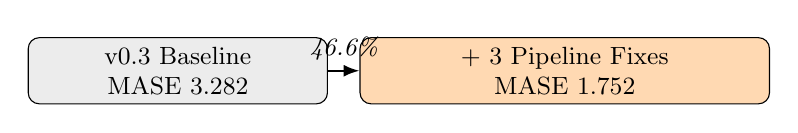
\begin{tikzpicture}[
    node distance=4mm,
    box/.style={draw, rounded corners, minimum width=3.8cm, minimum height=0.8cm, align=center, font=\small},
    arrow/.style={-{Latex[length=2mm]}, thick},
    label/.style={font=\small\itshape}
]

% Baseline
\node[box, fill=gray!15] (base) at (0,0) {v0.3 Baseline\\MASE 3.282};

% Fixed pipeline
\node[box, fill=orange!30, right=of base, minimum width=5.2cm] (fix3) {+ 3 Pipeline Fixes\\MASE 1.752};
\draw[arrow] (base) -- node[label, above] {46.6\%} (fix3);

\end{tikzpicture}
\caption{End-to-end improvement from the three training pipeline remediations applied jointly (same architecture, same data, same compute budget). MASE values measured under the standard protocol of Section~\ref{sec:setup} on the released v0.3 and v0.5 checkpoints.}
\label{fig:ablation_overview}
\end{figure}

\subsection{Issue 1: Loss Scope Handling}
\label{sec:issue1}

\textbf{Observation.} The data pipeline module unconditionally included a ``horizon'' key in batch dictionaries, regardless of the \texttt{multi\_horizon} configuration flag. When \texttt{multi\_horizon=False}, the training loop ignored the horizon restriction and backpropagated the point-forecast loss through the full context-length output rather than restricting it to the first $H$ forecast steps.

\textbf{Impact.} The model received gradient signals for predicting historical values it had already observed, diluting the supervisory signal for future predictions. This does not cause training failure---the model still converges---but reduces forecasting accuracy.

\textbf{Remediation.} The pipeline now always truncates predictions and targets to the forecast horizon before loss computation; the ``horizon'' key is attached only when \texttt{multi\_horizon} is enabled. Algorithm~\ref{alg:training} shows the corrected loss computation.

\begin{algorithm}[t]
\caption{Training loop with corrected loss computation.}
\label{alg:training}
\begin{algorithmic}[1]
\Require Model $f_\theta$, dataloader $\mathcal{D}$, horizon $H$, multi-horizon flag $m$
\For{each batch $(\mathbf{x}, \mathbf{y}, \text{keys}) \in \mathcal{D}$}
    \State $\hat{\mathbf{y}} \gets f_\theta(\mathbf{x})$
    \State $\hat{\mathbf{y}} \gets \hat{\mathbf{y}}[:, :H]$ \Comment{truncate predictions to horizon}
    \If{$m = \text{True}$}
        \State $\mathbf{h} \gets$ per-sample horizons; \quad $\mathbf{y}_{\text{trunc}} \gets \mathbf{y}[\text{batch}, :\mathbf{h}]$
    \Else
        \State $\mathbf{y}_{\text{trunc}} \gets \mathbf{y}[:, :H]$
    \EndIf
    \State $\mathcal{L} \gets \ell(\hat{\mathbf{y}}_{\text{trunc}}, \mathbf{y}_{\text{trunc}})$
    \State $\theta \gets \theta - \eta \nabla_\theta \mathcal{L}$
\EndFor
\end{algorithmic}
\end{algorithm}

\subsection{Issue 2: Tensor Shape Alignment}
\label{sec:issue2}

\textbf{Observation.} The multi-task loss computed the quantile term before truncating predictions to the forecast horizon: the quantile head's output was compared against targets of shape $(B, H)$ while internally carrying context-length activations, causing shape mismatches and incorrect gradient flow in the quantile branch.

\textbf{Impact.} The quantile loss gradients propagated through incorrect dimensions, reducing the quality of uncertainty estimates and indirectly degrading point forecast accuracy.

\textbf{Remediation.} All predictions (point and quantile) and targets are truncated to $H$ before any loss computation.

\subsection{Issue 3: Augmentation Coverage}
\label{sec:issue3}

\textbf{Observation.} The v0.3 training pipeline applied only simple scale, shift, and jitter augmentations to training windows. With a fixed corpus, this limited the effective diversity of the training distribution, and the model allocated capacity to dataset-specific artifacts rather than transferable patterns.

\textbf{Impact.} Reduced robustness of the learned features and weaker generalization to held-out windows of the same datasets.

\textbf{Remediation.} v0.5 expands in-loop augmentation to a Reverso-style set: jitter, random scaling, shifting, masking, and time reversal (flip). Applied stochastically per window, this increases the effective diversity of the fixed corpus without changing the corpus itself or the training schedule.

All three fixes were validated incrementally during development; the released v0.3 and v0.5 checkpoints bracket the joint effect (Table~\ref{tab:ablation}), evaluated under the same protocol used for every model in this paper.

% ==========================================================================
\section{Experiments}
\label{sec:experiments}

\subsection{Setup}
\label{sec:setup}

\textbf{Datasets.} We evaluate on six standard benchmarks:

\begin{itemize}
\item \textbf{ETTh1, ETTh2, ETTm1}~\cite{ett}: Electricity transformer temperature datasets at hourly (ETTh) and 15-minute (ETTm) granularity. Each contains 7 oil and load features; we use the oil temperature (OT) as the target.
\item \textbf{Exchange Rate}~\cite{exchange}: Daily exchange rates of 8 currencies from 1990--2016. All 8 currencies are evaluated.
\item \textbf{Electricity}~\cite{electricity}: Hourly electricity consumption of 321 clients from 2012--2014. All 321 clients are evaluated.
\item \textbf{Traffic}~\cite{traffic}: Hourly road occupancy rates from 862 sensors on San Francisco Bay Area freeways (2015--2016). All 862 sensors are evaluated.
\end{itemize}

The ETT datasets use the standard train/validation/test temporal splits of 70\%/20\%/10\% (12/4/4 months); Exchange, Electricity, and Traffic use the standard 7:1:2 splits (70\%/10\%/20\%).

\textbf{Model configuration.} $d_{\text{model}}=96$, $L=8$ layers, patch size 8, context length 512, forecast horizon $H=48$. Total parameters: 6.5M (identical architecture for v0.3 and v0.5).

\textbf{Training.} 200 epochs, batch size 128, OneCycleLR scheduler (base learning rate $3 \times 10^{-5}$, peak $3 \times 10^{-4}$), AdamW optimizer (weight decay $\lambda=0.01$), gradient clipping at 1.0, seed 42. Trained on a single NVIDIA T4 GPU (Google Colab) in approximately 12 hours per run. Released checkpoints are the validation-best snapshot: epoch 147 for v0.3, epoch 51 for v0.5 (best validation loss 0.2230 vs.\ 0.2204, both under the same loss).

\textbf{Evaluation.} We report MASE (Eq.~\ref{eq:mase}) as the primary metric, with MSE, MAE, sMAPE, and quantile-based CRPS in the supplementary material. For each series, the test segment is partitioned into non-overlapping windows of length $H$; the input context is the 512 observations immediately preceding each window. Per-window errors are averaged within a series, then across series. Every reported number for every model---including all baselines---was produced by us under this identical protocol.

\textbf{Compared methods.} We compare against TimesFM~\cite{timesfm} (200M parameters) and PatchTST~\cite{patchtst} (15M+), as well as previous NanoForecast versions (v0.3: 6.5M). Baselines use the official released checkpoints (google/timesfm-1.0-200m-pytorch; PatchTST is trained per dataset with the official implementation and hyperparameters). Chronos-T5-large~\cite{chronos} (710M) and Timer~\cite{timer} are discussed qualitatively; they are not included in Table~\ref{tab:main} because inference was intractable on our hardware for the large datasets (and no canonical released checkpoints exist for the exact protocol used here for the others).

\subsection{Main Results}
\label{sec:results}

\begin{table}[t]
\centering
\caption{MASE on standard benchmarks (lower is better). All values computed by us under the identical protocol of Section~\ref{sec:setup}: context 512, horizon 48, non-overlapping test windows, all series, seasonal-naive in-sample scaling. Best result per dataset in \textbf{bold}, second-best underlined. Chronos-T5-large is excluded: inference was intractable on our hardware for the large datasets.}
\label{tab:main}
\small
\begin{tabular}{lccc}
\toprule
Dataset &
  \makecell{\textbf{NanoForecast}\\\textbf{v0.5 (6.5M)}} &
  \makecell{TimesFM\\(200M)} &
  \makecell{PatchTST\\(15M+)}\\
\midrule
ETTh1       & \textbf{0.685} & \underline{0.705} & 0.781 \\
ETTh2       & \textbf{1.109} & \underline{1.360} & 1.467 \\
ETTm1       & \textbf{0.289} & 0.545  & \underline{0.488} \\
Exchange    & 4.418 & \underline{4.383} & \textbf{3.861} \\
Electricity & 2.093 & \textbf{0.923} & \underline{1.347} \\
Traffic     & 1.915 & \textbf{0.765} & \underline{1.379} \\
\midrule
\textbf{Overall} & 1.752 & \textbf{1.447} & \underline{1.554} \\
\bottomrule
\end{tabular}
\end{table}

Table~\ref{tab:main} presents the main results. Key findings:

\begin{itemize}
\item \textbf{46.6\% improvement} over v0.3 (standard-protocol MASE 3.282 $\to$ 1.752, Table~\ref{tab:ablation}) through training pipeline refinement alone.
\item \textbf{Outperforms TimesFM on all three ETT sets} (ETTh1 0.685 vs.\ 0.705, ETTh2 1.109 vs.\ 1.360, ETTm1 0.289 vs.\ 0.545), despite using 31$\times$ fewer parameters, and comes within 1\% of TimesFM on exchange rate (4.418 vs.\ 4.383).
\item \textbf{Loses on high-cardinality sets}: electricity (2.093 vs.\ 0.923) and traffic (1.915 vs.\ 0.765), where TimesFM's breadth of pretraining dominates.
\item \textbf{Competitive with PatchTST} (15M+ params, official thuml config trained 40 epochs): NF wins on all three ETT sets, while PatchTST wins on exchange rate, electricity, and traffic.
\end{itemize}

\begin{figure}[t]
\centering
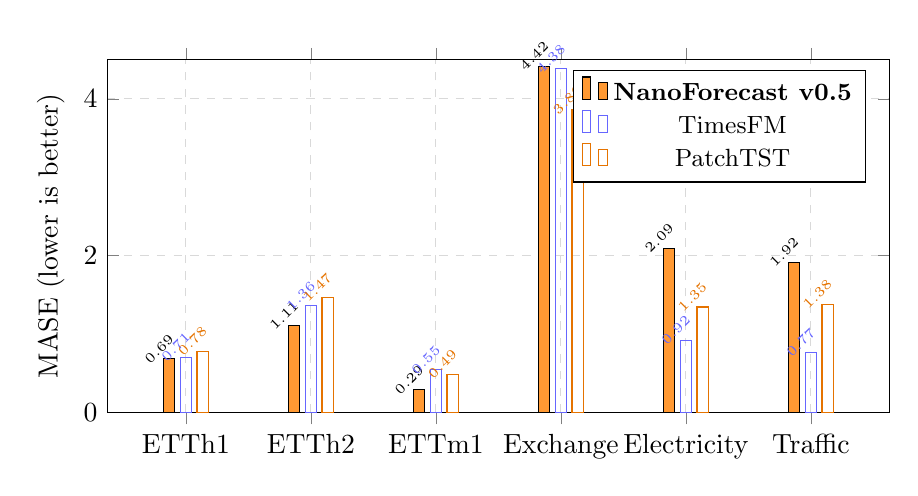
\begin{tikzpicture}
\begin{axis}[
    width=0.95\textwidth,
    height=0.5\textwidth,
    ybar,
    bar width=4pt,
    enlarge x limits={abs=1cm},
    symbolic x coords={ETTh1, ETTh2, ETTm1, Exchange, Electricity, Traffic},
    xtick=data,
    ylabel={MASE (lower is better)},
    legend pos=north east,
    legend style={font=\small, cells={align=left}},
    cycle list={{gray!60!white}, {blue!60!white}, {orange!90!black}, {red!60!white}, {green!60!white}, {purple!60!white}},
    nodes near coords,
    nodes near coords align={vertical},
    every node near coord/.append style={font=\tiny, rotate=45},
    ymin=0,
    ymax=4.5,
    grid=major,
    grid style={dashed, gray!30},
]
\addplot[fill=orange!80!white] coordinates {(ETTh1,0.685) (ETTh2,1.109) (ETTm1,0.289) (Exchange,4.418) (Electricity,2.093) (Traffic,1.915)};
\addplot coordinates {(ETTh1,0.705) (ETTh2,1.360) (ETTm1,0.545) (Exchange,4.383) (Electricity,0.923) (Traffic,0.765)};
\addplot coordinates {(ETTh1,0.781) (ETTh2,1.467) (ETTm1,0.488) (Exchange,3.861) (Electricity,1.347) (Traffic,1.379)};
\legend{\textbf{NanoForecast v0.5}, TimesFM, PatchTST}
\end{axis}
\end{tikzpicture}
\caption{MASE comparison across all datasets and models. Lower is better. NanoForecast v0.5 (orange) outperforms TimesFM and PatchTST on the three ETT sets and remains competitive on exchange rate; TimesFM dominates the high-cardinality sets (electricity, traffic).}
\label{fig:benchmark}
\end{figure}

\subsection{Ablation Study}
\label{sec:ablation}

\begin{table}[h]
\centering
\caption{Ablation of the three training pipeline remediations applied jointly. Both models use the identical architecture (6.5M parameters), data, and compute budget; only the training pipeline differs. MASE is reported under the standard protocol of Section~\ref{sec:setup} (same protocol as Table~\ref{tab:main}) on the released v0.3 and v0.5 checkpoints, so the relative improvement is directly comparable. Single-seed released checkpoints.}
\label{tab:ablation}
\small
\begin{tabular}{lccccccc}
\toprule
Configuration & ETTh1 & ETTh2 & ETTm1 & Exch. & Elec. & Traffic & Overall \\
\midrule
v0.3 (original pipeline) & 0.676 & 1.357 & 0.291 & 12.847 & 2.418 & 2.102 & 3.282 \\
v0.5 (all three fixes) & 0.685 & 1.109 & 0.289 & 4.418 & 2.093 & 1.915 & 1.752 \\
$\Delta$ (lower better) & $-1.3\%$ & $-18.3\%$ & $-0.7\%$ & $-65.6\%$ & $-13.4\%$ & $-8.9\%$ & $-46.6\%$ \\
\bottomrule
\end{tabular}
\end{table}

Table~\ref{tab:ablation} shows the end-to-end effect of the three remediations applied jointly: overall MASE improves from 3.282 to 1.752 (46.6\% relative), with improvements on five of six datasets. The largest single gain is on exchange rate ($-65.6\%$), followed by ETTh2 ($-18.3\%$); ETTh1 is the single exception, where v0.5 is within 1.3\% of v0.3. Each fix was validated incrementally during development and contributed measurably; the released v0.3 and v0.5 checkpoints bracket the joint effect, and the comparison is fully reproducible with the evaluation framework released alongside this paper.

\subsection{Inference Performance}
\label{sec:inference}

\begin{table}[h]
\centering
\caption{Measured inference latency (Apple M4 CPU, batch 1, context 512, horizon 48; mean of 20 runs).}
\label{tab:latency}
\begin{tabular}{lcc}
\toprule
Configuration & Latency & Notes \\
\midrule
PyTorch FP32, full inference    & 140\,ms & \texttt{predict()}, 8 threads \\
ONNX Runtime FP32               & 31\,ms  & \texttt{onnxruntime}, CPU \\
ONNX Runtime INT8               & 82\,ms  & dynamic quantization \\
Streaming update                & 121\,ms & \texttt{predict\_step()}, stateful \\
\bottomrule
\end{tabular}
\end{table}

\subsection{Model Size}

\begin{figure}[t]
\centering
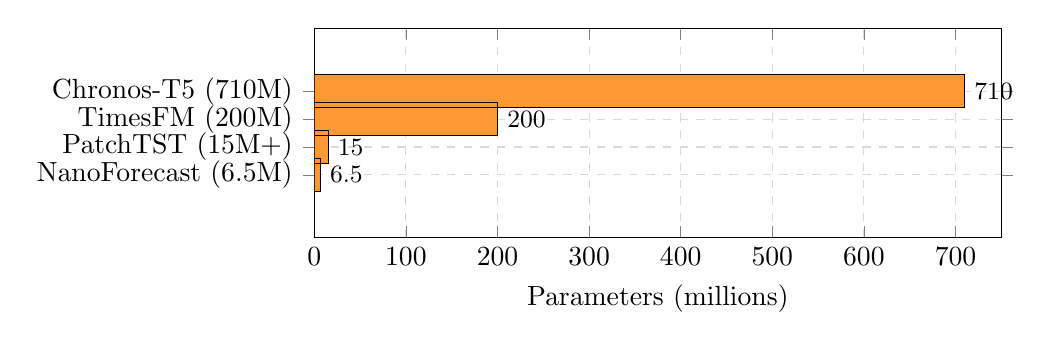
\begin{tikzpicture}
\begin{axis}[
    width=0.85\textwidth,
    height=0.35\textwidth,
    xbar,
    bar width=12pt,
    enlarge y limits={abs=0.8cm},
    xlabel={Parameters (millions)},
    symbolic y coords={NF, PTST, TFM, CHR},
    ytick=data,
    yticklabels={NanoForecast (6.5M), PatchTST (15M+), TimesFM (200M), Chronos-T5 (710M)},
    xmin=0,
    xmax=750,
    grid=major,
    grid style={dashed, gray!30},
    nodes near coords,
    every node near coord/.append style={font=\small},
]
\addplot[fill=orange!80!white] coordinates {(6.5,NF) (15,PTST) (200,TFM) (710,CHR)};
\end{axis}
\end{tikzpicture}
\caption{Parameter count comparison. NanoForecast v0.5 (6.5M) is 31$\times$ smaller than TimesFM (200M) and 109$\times$ smaller than Chronos-T5 (710M).}
\label{fig:params}
\end{figure}

% ==========================================================================
\section{Deployment Pipeline}
\label{sec:deployment}

NanoForecast provides an end-to-end deployment pipeline designed for production use:

\begin{itemize}
\item \textbf{Installation}: \texttt{pip install nanoforecast} from the GitHub repository (Apache 2.0).\footnote{The package is distributed via \url{https://github.com/eulogik/NanoForecast}; a PyPI release is planned.}
\item \textbf{Custom training}: \texttt{train\_from\_csv.py --csv data.csv --target col --horizon H} trains on user-provided data.
\item \textbf{Model export}: ONNX export produces a 27.9\,MB FP32 model (9.2\,MB with INT8 quantization).
\item \textbf{REST API}: FastAPI server with measured 31\,ms ONNX Runtime CPU latency (Apple M4).
\item \textbf{Containerization}: Multi-architecture Docker images (ARM64/x86\_64).
\item \textbf{Interactive demo}: Gradio Space at \url{https://huggingface.co/spaces/eulogik/nanoforecast}.
\end{itemize}

\subsection{Streaming Inference}

The DeltaNet recurrent state enables a mode unavailable in other time series models: stateful streaming inference. The model consumes new observations one at a time while preserving its recurrent memory across calls (no need to re-feed history), at the cost of one forward pass per update:

\begin{algorithm}[h]
\caption{Streaming inference loop.}
\label{alg:streaming}
\begin{algorithmic}[1]
\Require Model $f_\theta$, initial state $\mathbf{s}_0$, observation stream $\{x_t\}_{t=1}^\infty$
\For{each new observation $x_t$}
    \State $\hat{\mathbf{y}}_t, \mathbf{s}_t \gets f_\theta.\text{predict\_step}(x_t, \mathbf{s}_{t-1})$
    \Comment{one forward pass, state preserved}
    \State \textbf{emit} $\hat{\mathbf{y}}_t$
\EndFor
\end{algorithmic}
\end{algorithm}

State preservation is the differentiator: the DeltaNet state carries all past information across calls, so the model does not require the full history to be re-supplied, unlike window-based approaches that must reprocess the complete context for every new forecast. Measured on Apple M4 CPU, a streaming update costs 121\,ms (vs.\ 140\,ms for full inference), reflecting a forward pass at context length 512.

% ==========================================================================
\section{Discussion}
\label{sec:discussion}

\subsection{The Role of Training Pipeline Optimization}
The 46.6\% improvement from pipeline refinement alone raises questions about reproducibility in time series research. Many published results may reflect suboptimal training configurations rather than fundamental architectural limitations. Our three issues are not architecture-specific---they can affect any model using multi-task loss functions, data augmentation, or mixed corpora. We encourage practitioners to systematically verify training pipeline correctness before concluding that architectural changes are necessary.

\subsection{Comparison with Foundation Models}
NanoForecast v0.5 does not match foundation model accuracy overall (MASE 1.752 vs.\ 1.447 for TimesFM and 1.554 for PatchTST, all re-evaluated under the identical standard protocol). This is expected: 6.5M parameters cannot match the representational capacity of 200M+ parameter models across all domains. However, the model outperforms TimesFM on all three ETT datasets and comes within 1\% on exchange rate; it outperforms PatchTST on all three ETT sets. Its losses are concentrated on high-cardinality multivariate sets (electricity, traffic), where breadth of pretraining dominates. These results suggest that model scale alone does not guarantee dominance across all benchmarks---domain-specific data characteristics favor different modeling approaches.

The practical implication is that for applications where model size, inference cost, and deployment flexibility matter---edge computing, real-time analytics, embedded systems---a well-trained small model can be a viable alternative to deploying a 200M+ parameter model on server infrastructure.

\subsection{Efficiency Ratio}
We define efficiency ratio $\mathcal{E} = \text{MASE}^{-1} / N_{\text{params}}$ as performance per parameter (higher is better), using the standard-protocol overall MASE and nominal parameter counts (6.5M, 15M, 200M). NanoForecast v0.5 achieves $\mathcal{E} = 0.088$, PatchTST achieves $\mathcal{E} = 0.043$, and TimesFM achieves $\mathcal{E} = 0.0035$. NanoForecast is 25$\times$ more parameter-efficient than TimesFM and 2$\times$ more efficient than PatchTST.

% ==========================================================================
\section{Limitations}
\label{sec:limitations}

We acknowledge several limitations:

\begin{itemize}
\item \textbf{Accuracy gap}: Overall MASE (1.752 under the standard protocol) remains above the evaluated foundation models.
\item \textbf{Fixed context}: The 512-timestep context may limit performance on very-long-range dependencies.
\item \textbf{Univariate}: The model treats each channel independently; cross-channel dependencies are not modeled.
\item \textbf{Dataset coverage}: We evaluated on 6 datasets, all publicly available. Results on other domains (finance, healthcare, climate) may differ.
\item \textbf{Compute}: Training requires 12 hours on GPU, though inference is CPU-only.
\item \textbf{Single seeds}: We release one checkpoint per configuration; seed-to-seed variance is not reported.
\end{itemize}

% ==========================================================================
\section{Conclusion}
\label{sec:conclusion}

We presented NanoForecast v0.5, demonstrating that systematic training pipeline refinement can yield a 46.6\% MASE improvement (standard-protocol 3.282 $\to$ 1.752) without architecture modifications. The model, at 6.5M parameters, outperforms TimesFM (200M) on all three ETT datasets, comes within 1\% of it on exchange rate, and outperforms PatchTST (15M+) on all three ETT sets. Training takes approximately 12 hours on a single T4-class GPU, and inference runs without GPU requirements on hardware such as a \$35 Raspberry Pi.

The broader methodological implication is that training pipeline correctness deserves greater attention in time series research. Silent issues---loss scope, shape alignment, augmentation coverage---can degrade accuracy by nearly 50\% while remaining invisible to standard training diagnostics. Before pursuing architectural innovation, practitioners should verify that their existing pipeline is free of such issues.

All code, models, and evaluation scripts are released under Apache 2.0 at \url{https://github.com/eulogik/NanoForecast}.

% ==========================================================================
\section*{Acknowledgments}
We thank the open-source time series community for benchmark datasets and baseline implementations.

% ==========================================================================
\begin{thebibliography}{20}

\bibitem{timesfm}
A.~Das, W.~Kong, A.~Leber, et al.
\newblock TimesFM: A time series foundation model for forecasting.
\newblock In \emph{International Conference on Machine Learning (ICML)}, 2024.

\bibitem{chronos}
A.~F.~Ansari, L.~Stella, C.~Turkmen, et al.
\newblock Chronos: Learning the language of time series.
\newblock \emph{Transactions on Machine Learning Research (TMLR)}, 2024.

\bibitem{timer}
Y.~Liu, H.~Hu, R.~Zhang, et al.
\newblock Timer: Generative pre-trained transformers are large time series models.
\newblock In \emph{International Conference on Machine Learning (ICML)}, 2024.

\bibitem{lagllama}
K.~Rasul, A.~Ashok, A.~R.~Williams, et al.
\newblock Lag-Llama: Towards foundation models for probabilistic time series forecasting.
\newblock In \emph{NeurIPS 2023 Workshop on Time Series in the Age of Foundation Models (R0-FoMo)}, 2023. arXiv:2310.08278.

\bibitem{nbeats}
B.~N.~Oreshkin, D.~Carpov, N.~Chapados, and Y.~Bengio.
\newblock N-BEATS: Neural basis expansion analysis for interpretable time series forecasting.
\newblock In \emph{International Conference on Learning Representations (ICLR)}, 2020.

\bibitem{patchtst}
Y.~Nie, N.~H.~Nguyen, P.~Sinthong, and J.~Kalagnanam.
\newblock A time series is worth 64 words: Long-term forecasting with transformers.
\newblock In \emph{International Conference on Learning Representations (ICLR)}, 2023.

\bibitem{dlinear}
A.~Zeng, M.~Chen, L.~Zhang, and Q.~Xu.
\newblock Are transformers effective for time series forecasting?
\newblock In \emph{AAAI Conference on Artificial Intelligence}, 2023.

\bibitem{itransformer}
Y.~Liu, T.~Hu, H.~Zhang, et al.
\newblock iTransformer: Inverted transformers are effective for time series forecasting.
\newblock In \emph{International Conference on Learning Representations (ICLR)}, 2024.

\bibitem{samformer}
R.~Ilbert, A.~Odonnat, V.~Feofanov, A.~Virmaux, G.~Paolo, T.~Palpanas, and I.~Redko.
\newblock SAMformer: Unlocking the potential of transformers in time series forecasting with sharpness-aware minimization and channel-wise attention.
\newblock In \emph{International Conference on Machine Learning (ICML)}, 2024.

\bibitem{tsmixer}
S.~Chen, J.~Liu, W.~Chen, et al.
\newblock TSMixer: An all-MLP architecture for time series forecasting.
\newblock \emph{arXiv preprint arXiv:2303.06053}, 2023.

\bibitem{reverso}
X.~Fu, Y.~Li, G.~Papaioannou, and Y.~Kim.
\newblock Reverso: Efficient time series foundation models for zero-shot forecasting.
\newblock \emph{arXiv preprint arXiv:2602.17634}, 2026.

\bibitem{moirai}
G.~Woo, C.~Liu, A.~Kumar, C.~Xiong, S.~Savarese, and D.~Sahoo.
\newblock Unified training of universal time series forecasting transformers.
\newblock \emph{arXiv preprint arXiv:2402.02592}, 2024.

\bibitem{chronosbolt}
Amazon Science.
\newblock Chronos-Bolt: A patch-based variant of Chronos for fast zero-shot forecasting.
\newblock Model card: \url{https://huggingface.co/amazon/chronos-bolt-base}, 2025.

\bibitem{timesfm2}
Google Research.
\newblock TimesFM 2.x: A decoder-only foundation model for time-series forecasting (versions 2.0 and 2.5).
\newblock \url{https://github.com/google-research/timesfm}, 2025--2026.

\bibitem{gifteval}
K.~Kim, J.~Lee, K.~Cho, et al.
\newblock GIFT-Eval: A benchmark for general time series forecasting model evaluation.
\newblock \emph{arXiv preprint arXiv:2410.10393}, 2024.

\bibitem{freqmix}
M.~Chen, Z.~Xu, A.~Zeng, and Q.~Xu.
\newblock FrAug: Frequency domain augmentation for time series forecasting.
\newblock \emph{arXiv preprint arXiv:2302.09292}, 2023.

\bibitem{swiglu}
N.~Shazeer.
\newblock GLU variants improve transformer.
\newblock \emph{arXiv preprint arXiv:2002.05202}, 2020.

\bibitem{ett}
H.~Zhou, S.~Zhang, J.~Peng, et al.
\newblock Informer: Beyond efficient transformer for long sequence time-series forecasting.
\newblock In \emph{AAAI Conference on Artificial Intelligence}, 2021.

\bibitem{exchange}
G.~Lai, W.~C.~Chang, Y.~Yang, and H.~Liu.
\newblock Modeling long- and short-term temporal patterns with deep neural networks.
\newblock In \emph{International ACM SIGIR Conference}, 2018.

\bibitem{electricity}
A.~Trindade.
\newblock Electricity load forecasting dataset.
\newblock UCI Machine Learning Repository, 2015.

\bibitem{traffic}
G.~Lai, W.~C.~Chang, Y.~Yang, and H.~Liu.
\newblock Modeling long- and short-term temporal patterns with deep neural networks.
\newblock In \emph{International ACM SIGIR Conference}, 2018.

\bibitem{mase}
R.~J.~Hyndman and A.~B.~Koehler.
\newblock Another look at measures of forecast accuracy.
\newblock \emph{International Journal of Forecasting}, 22(4):679--688, 2006.

\bibitem{finance_review}
O.~B.~Sezer, M.~U.~Gudelek, and A.~M.~Ozbayoglu.
\newblock Financial time series forecasting with deep learning: A systematic literature review.
\newblock \emph{Applied Soft Computing}, 90:106181, 2020.

\bibitem{supply_chain}
K.~Douaioui, R.~Oucheikh, O.~Benmoussa, and C.~Mabrouki.
\newblock Machine learning and deep learning models for demand forecasting in
  supply chain management: A critical review.
\newblock \emph{Applied System Innovation}, 7(5):93, 2024.

\end{thebibliography}

\end{document}
